\documentclass[proyecto.tex]{subfiles}

\begin{document}

\noindent\textbf{Propuesta de proyecto:}

\bigskip

\noindent\begin{tabularx}{\textwidth}{|>{\columncolor{tcc}}X|}
\hline
En esta sección, explique en detalle los siguientes aspectos:
\begin{enumerate}[label={\alph*)},nosep]
\item Problema a resolver o aplicación a desarrollar.
\item Objetivos de trabajo.
\item Metodología de trabajo y herramientas disponibles para cumplir los objetivos.
\item Plan de trabajo o carta gantt.
\end{enumerate}

\medskip

Número máximo de palabras en esta sección: \textbf{1500 palabras}.\\
\hline
\end{tabularx}

%%%%%%%%%%%%%%%%%%%%%%%%%%%%%%%%%%%%%%%%%%%%%%%%%%%%%%%%%%%%%%%%%%%%%%%%%%%%%%%%
\section{Problema a resolver o aplicación a desarrollar}

\begin{figure}[h!]
    \centering
    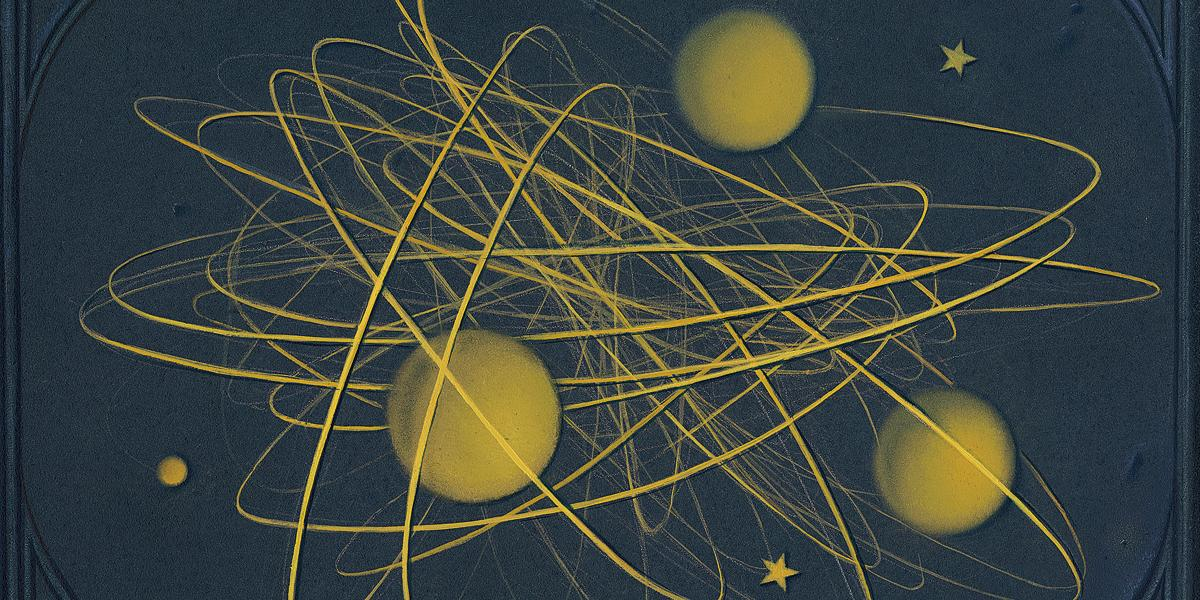
\includegraphics[width=8cm]{articleImage-big.jpg}
    \caption{Ilustración de Chris Bruzelli del problema de los 3 cuerpos \cite{bruzelli}}
    \label{fig:bruzelli}
\end{figure}

\ Desde que Newton planteó la Ley de la Gravitación Universal, se han derivado distintos cuestionamientos acerca de casos aplicados a la realidad, en particular, nuestro equipo se interesó en uno de los más controversiales problemas y posiblemente el con más aplicaciones para, por ejemplo, lanzamientos espaciales o estudios de sistemas planetarios. Hablamos del reconocido \textbf{problema de los 3 cuerpos}, el cual, como muchos ya saben, consiste en encontrar las trayectorias u orbitas en todo instante de tiempo de tres masas sometidas a una interacción gravitatoria mútua. Parece no tener mayores complicaciones en su resolución, ya que si recordamos lo que nos dice la Segunda Ley de Newton y su Ley de Gravitación Universal respectivamente:

\begin{align}
    \vec{F_{ij}} &= m_{i}\vec{x_{i}}'' = m_{i}\vec{a_i}; \label{eq:2leyN} \\
    \vec{F} &= \frac{GMm}{r^2}\hat{r},
\end{align}

\noindent aparenta ser relativamente intuitivo el desarrollo del despeje de las trayectorias de los cuerpos mediante ecuaciones diferenciales, pero no es así. Este problema lleva vigente más de un siglo e increíblemente no se han podido encontrar las soluciones analíticas, pero es aquí donde emerge nuestra área de interés, las \textit{soluciones numéricas}. Cuando se plantean las ecuaciones diferenciales del problema, lo matemáticos se encontraron un problema que presentaba más incógnitas que ecuaciones, por lo que con el pasar de los años, se fueron desarrollando distintos métodos para llegar a soluciones que se aproximaran lo bastante bien a los comportamientos físicos que se interpretan de las formas de las ecuaciones, en particular, los \textit{métodos numéricos} se llevaron el papel fundamental en este desarrollo. Actualmente, las soluciones computacionales y simulaciones derivadas de los métodos ya mencionados, han logrado gracias a sus excelentes aproximaciones , lanzar misiones como \textit{el Telescopio Espacial Hubble} o \textit{el Telescopio Espacial SPITZER}, los cuales, entre muchos otros, han requerido de distintas soluciones al \textit{prroblema de los 3 cuerpos} para predecir las trayectorias al ser lanzados a órbita.

\par En nuestro estudio de este problema, partiremos con el análisis de \textbf{el problema de los 2 cuerpos} (lo mismo pero con un cuerpo menos), el cual si tiene solución analítica, por lo que se buscará en primera instancia estas trayectorias u orbitas. También, estudiaremos \textbf{las soluciones particulares de Euler y Lagrange} al problema de los 3 cuerpos, las cuales disponen las masas en ciertas posiciones geométricas que permiten simplificar el problema y encontrar las soluciones. Luego, procederemos a abordar directamente el problemas de los 3 cuerpos, partiendo con un desarrollo analítico, con la intención de comprender el por qué no tiene solución analítica, para luego abordar algunas soluciones numéricas mediante \textbf{simulaciones}, y por último, se buscará la manera de \textbf{animar} algunas de estas en \textbf{2D} y \textbf{3D}, para una visualización del comportamiento caótico de los 3 cuerpos.



%%%%%%%%%%%%%%%%%%%%%%%%%%%%%%%%%%%%%%%%%%%%%%%%%%%%%%%%%%%%%%%%%%%%%%%%%%%%%%%%
\section{Objetivos de trabajo}

\subsection{Objetivo general}

\par Simular mediante animaciones 2D y 3D algunos casos particulares del problema de los 3 cuerpos.

\subsection{Objetivos específicos}
\begin{enumerate}
\item Introducir al lector sobre el problema a desarrollar, y familiarizarlo con la física que se ocupará.
\item Resolver analíticamente el problema de los 2 cuerpos. 
\item Resolver numéricamente el problema de los 2 cuerpos.
\item Comparar gráficamente soluciones numéricas con la analítica del problema de los 2 cuerpos.
\item Formular analíticamente el problema de los 3 cuerpos para comprender su imposibilidad de solucionarlo por esta vía.
\item Estudiar las soluciones particulares impuestas por Euler y posteriormente por Lagrange al problema de los 3 cuerpos.
\item Resolver numéricamente algunos casos del problema de los 3 cuerpos.
\item (Objetivo general) Simular mediante animaciones 2D y 3D algunos casos particulares del problema de los 3 cuerpos.
\end{enumerate}

\section{Metodología} \label{item:c}

\begin{enumerate}
\item Para introducir al lector sobre el problema de los 3 cuerpos , se investigará en base a la bibliografía planteada sobre su historia y aplicaciones. Además, se introducirá la traducción matemática que definen a los problemas (ecuaciones diferenciales) y se plantearán algunas leyes de la \textit{mecánica de Newton} y de la \textit{mecánica de Hamilton-Jacobi}. Por último, se describirán los métodos numéricos para la resolución de ecuaciones diferenciales: el \textit{método de Runge-Kutta} y el \textit{método de Euler}.
\item Para la resolución analítica del problema de los 2 cuerpos,se desarrollará a partir de la Segunda Ley de Newton y de la Ley de Gravitación Universal, ocupando herramientas matemáticas como un sistema de coordenadas en el plano complejo y métodos analíticos de resolución de ecuaciones diferenciales.
\item Para la resolución numérica del problema de los 2 cuerpos, se ocuparán 2 métodos para la resolución de ecuaciones diferenciales, el \textit{método de Runge-Kutta} y el \textit{método de Euler} en el lenguaje de Python en un ordenador de 64 bits, definiendo los métodos en en ciclo \textit{for} generalizado y definiendo por otro lado las ecuaciones diferenciales a resolver con sus respectivas condiciones iniciales, agregando también, que se hará uso del módulo \textit{numpy} de \textit{Python}.
\item Para hacer la comparación gráfica, se utilizará el lenguaje de programación \textit{Python}, donde se ocuparán los módulos \textit{matplotlib.pyplot} y \textit{numpy}. Para ello, se tomarán las soluciones analíticas resultantes para el problema de los 2 cuerpos y las soluciones numéricas obtenidas tanto con el \textit{método de Runge-Kutta} como con el \textit{método de Euler}, y se graficarán con el módulo \textit{matplotlib.pyplot} de \textit{Python}, de manera que al analizar los gráficos se haga una discriminación del método numérico que mejor se aproxima a la solución analítica real.
\item Para la formulación analítica del problema central a abordar (el problema de los 3 cuerpos), se hará un desarrollo inicial análogo al que se hizo con la solución analítica del problema de los 2 cuerpos, explicando al final porque no se puede continuar con el cálculo.
\item Para hacer el estudio de las soluciones particulares a los problemas restringidos de los tres cuerpos de Euler y Lagrange (soluciones colineales y triangulares respectivamente), se investigarán en base a una bibliografía que se especificará y se estudiarán los gráficos de estas soluciones.
\item Para el último objetivo, se resolverán algunos casos particulares al problema de los tres cuerpos, que se especificarán al momento de realizarlo, donde se utilizarán nuevamente los \textit{métodos de Runge-Kutta y de Euler} en el lenguaje de programación \textit{Python}. 
\item Luego de obtener estas soluciones, serán simuladas en 2D y 3D con el módulo \textit{matplotlib.animation} en conjunto con módulos más incidentales para este caso como \textit{matplotlib.pyplot} y \textit{numpy}. Cabe recalcar, que las simulaciones serán atribuídas a los artículos \cite{Musielak_2014,simulation3d,Iker_2017}, con el propósito de unificar un código traducido al lenguaje de programación de \textit{Python} en un ordenador de 64 bits.
\end{enumerate}

\section{Plan de trabajo y carta Gantt}

\par Luego de haber aclarado la metodología, nos queda sólo organizar el ''itinerario" de prácticas para llevar a cabo el proyecto. Para ello, enumeraremos una lista espedita de tareas que permitirán concretar los objetivos específicos ya mencionados, para luego llevarlos una ''diagrama temporal'' en forma de una \textit{carta de Gantt}, donde se puntualizarán los objetivos que se esperan lograr por semana mediante las tareas que posibilitarán precisamente alcanzar los objetivos en un tiempo determinado. 

\par Las tareas que se llevarán a cabo para lograr cada objetivo son:

\begin{enumerate}
    \item \textbf{Para el objetivo 1:}
    
    \par Se investigará sobre el problema de los 3 cuerpos con la bibliografía planteada; se estudiarán los métodos tanto físicos, matemáticos y numéricos que serán necesarios para el desarrollo; se extraerá lo esencial de lo recién mencionado en una sección introductoria para el proyecto.
    
    \item \textbf{Para el objetivo 2:}
    
    \par Se plantearán las ecuaciones diferenciales para la resolución analítica del problema de los 2 cuerpos; se resolverán estas ecuaciones con lo métodos ya indicados en la sección \ref{item:c} para distintas condiciones iniciales.
    
    \item \textbf{Para el objetivo 3:}
    
    \par Se plantearán las ecuaciones diferenciales para resolver el problema de los 2 cuerpos; se traducirán estas ecuaciones al lenguaje de programación \textit{Python}; se resolverá numéricamente el problema de los 2 cuerpos con los métodos indicados en la sección \ref{item:c} en \textit{Python} para distintas condiciones iniciales.
    
    \item \textbf{Para el objetivo 4:}
    
    \par Se graficarán en \textit{Python} las soluciones analíticas y numéricas del problema de los 2 cuerpos; se compararán entre ellas para encontrar el método numérico que mejor se aproxima a la solución analítica.
    
    \item \textbf{Para el objetivo 5:}
    
    \par Se plantearán las ecuaciones diferenciales que hipotéticamente permiten resolver analíticamente el problema de los 3 cuerpos; se explicarán las limitaciones matemáticas que impiden resolver analíticamente este problema.
    
    \item \textbf{Para el objetivo 6:}
    
    \par Se investigará sobre las soluciones particulares que descubrieron Euler y Lagrange; se hará tanto un estudio como un análisis de estas soluciones; se agregarán tanto links, como imágenes para comprender visualmente estas soluciones.
    
    \item \textbf{Para el objetivo 7:}
    
    \par Se plantearán las ecuaciones diferenciales para resolver el problema de los 3 cuerpos; se traducirán estas ecuaciones al lenguaje de programación \textit{Python}; se resolverán numéricamente algunos casos del problema de los 3 cuerpos con los métodos indicados en la sección \ref{item:c} en \textit{Python} para distintas condiciones iniciales.
    
    \item \textbf{Para el objetivo 8 (objetivo general):}
    
    \par Se ocuparán las soluciones encontradas numéricamente al problema de los 3 cuerpos para simular mediante animaciones en 2D y 3D las trayectorias de los 3 cuerpos con los métodos indicados en la sección \ref{item:c}.
    
\end{enumerate}

\par Así, considerando que nuestros objetivos fueros planteados secuencialmente, podemos organizar una carta de Gantt que indicará los tiempos necesarios para cumplir cada objetivo específico (considerando las tareas recién mencionadas), donde se dispondrán de 5 semanas para alcanzar el objetivo general, 2 de noviembre y 3 de diciembre. Entonces el itinerario nos queda de la siguiente forma:

% example adapted from https://tex.stackexchange.com/questions/587422/draw-gantt-chart-latex-with-pgfgantt/587449#587449
\begin{center}
  \begin{ganttchart}[vgrid, hgrid, 
    y unit title=0.5cm,
    y unit chart=0.5cm,
    x unit=2.5cm,
    title height=1,
    progress label text={},
    bar height=0.5 ]{1}{5}   % divide la tabla en 8 columnas. 
    % Esta carta gantt está dividida en 8 semanas (2 meses). Cada
    % columna representa una semana.

    % periodos
    \gantttitle{2021}{5} \\ % titulo usa 8 columnas
    \gantttitle{Noviembre}{2} \gantttitle{Diciembre}{3} \\ % 2 titulos, cada uno usa 4 columnas

    % tareas
    \ganttbar[progress=25, name=obj1]{Objetivos 1, 2, 3 y 4}{1}{1} \\  % actividad se realiza entre las semanas 1-2; lleva 30% de progreso
    \ganttbar[progress=0, name=obj2]{Objetivo 5}{2}{3} \\  % actividad entre las semanas 3-5, 50% de progreso
    \ganttbar[progress=0, name=obj3 ]{Objetivo 6}{3}{4} \\ % actividad entre semanas 4-7, aun no inicia
    \ganttbar[progress=0, name=obj4]{Objetivos 7 y 8}{4}{5}          % actividad entre semanas 6-8, aun no inicia
    
    %relations 
    %\ganttlink{obj1}{obj3} % relaciona las tareas que definen 'name' (obj3 depende de obj1)
  \end{ganttchart}
\end{center}


% lista de referencias guardadas en referencias.bib

\bibliographystyle{amsplain}
\bibliography{referencias}

\end{document}
